% ============================================================================
% Expérience 01 — Instabilité bootstrap (Fang & Wang, 2012) / nselectboot
% Compilation : make (depuis ce dossier)
% ============================================================================

\documentclass[11pt, a4paper]{article}
\usepackage[utf8]{inputenc}
\usepackage[T1]{fontenc}
\usepackage[french]{babel}
\usepackage{amsmath, amssymb}
\usepackage[margin=2.5cm]{geometry}
\usepackage{booktabs}
\usepackage{float}
\usepackage{graphicx}
\usepackage{xcolor}
\usepackage{hyperref}
\hypersetup{colorlinks=true, linkcolor=blue}

% Heatmaps simulées : \HeatmapSim{S1}{1} → fichier figures/nselectboot_heatmap_sim_S1_seed1.png
\newcommand{\HeatmapSim}[2]{%
\IfFileExists{figures/nselectboot_heatmap_sim_#1_seed#2.png}{%
\begin{center}
\includegraphics[width=0.85\textwidth]{figures/nselectboot_heatmap_sim_#1_seed#2.png}
\end{center}}{%
\begin{center}
\textit{(Figure absente : \texttt{nselectboot\_heatmap\_sim\_#1\_seed#2.png} — exécuter
\texttt{run\_nselectboot\_simulated.R} puis \texttt{analyse\_nselectboot\_simulated.R}.)}
\end{center}}}

\title{Rapport d'instabilité --- Expérience 01 (Fang \& Wang)}
\author{Pierre Chambet}
\date{Mars 2026}

\begin{document}
\maketitle

\begin{abstract}
On veut choisir $k$ (nombre de clusters) et les paramètres de distance
$(\alpha,\omega)$ sans labels. Ce rapport se concentre sur une méthode de la
littérature : \textbf{nselectboot} (Fang \& Wang, 2012), implémentée dans R
(\texttt{fpc::nselectboot}), qui minimise une \textbf{instabilité} mesurée par
bootstrap. Un ancien protocole de « stabilité » ad hoc (sans article de référence)
a été retiré pour clarifier le message. On teste une grille 21×21 en
$(\alpha,\omega)$ sur quatre jeux de données ; les labels ne servent qu'à
évaluer l'ARI une fois $k$ choisi. Un \textbf{volet simulé} (données hybrides Cas2\_deriv, aligné sur l'expérience~03)
complète l'étude sous vérité de $k$ connue. Les figures et CSV simulés versionnés
ici proviennent du \textbf{mode rapide} (grille $6\times6$, $B=60$) pour un coût
raisonnable ; les quatre jeux réels restent en grille $21\times21$, $B=150$.
\end{abstract}

\tableofcontents
\newpage

% ============================================================================
\section{Objectif de l'expérience 1}
% ============================================================================

On veut choisir trois quantités \textbf{sans utiliser les labels pour le choix} :

\begin{itemize}
  \item \textbf{$k$} : nombre de clusters.
  \item \textbf{$\alpha$} : pondération entre distance sur les courbes (niveau)
    et sur les dérivées (forme).
  \item \textbf{$\omega$} : pondération entre partie fonctionnelle et partie
    vectorielle ($Z$).
\end{itemize}

La méthode retenue est \textbf{nselectboot} : pour chaque couple $(\alpha,\omega)$
de la grille, on estime un $k_\text{opt}$ qui minimise l'instabilité bootstrap.
On obtient une carte $(\alpha,\omega) \mapsto k_\text{opt}$ et des heatmaps
d'instabilité par $k$.

\paragraph{Pourquoi une grille en $(\alpha,\omega)$ ?}
Parce que $\alpha$ et $\omega$ changent la matrice de distances $D_w(\alpha,\omega)$
et donc le clustering. Les heatmaps montrent l'instabilité par $(\alpha,\omega)$
et $k$ : \textbf{bleu = faible instabilité (bon)}, \textbf{rouge = forte (mauvais)}.

% ============================================================================
\section{Le problème en une phrase}
% ============================================================================

Pour du clustering, il faut fixer $k$ et la distance. Sans vérité terrain pour
choisir, on utilise un critère documenté (instabilité bootstrap).

% ============================================================================
\section{Les trois paramètres et les données}
% ============================================================================

\begin{itemize}
  \item \textbf{$k$} : nombre de clusters testé dans $\{2,\ldots,6\}$.
  \item \textbf{$\alpha$} : mélange $D_0$ (courbes) / $D_1$ (dérivées).
  \item \textbf{$\omega$} : mélange distance fonctionnelle / distance sur $Z$.
\end{itemize}

Quatre jeux de données (labels uniquement pour \textbf{évaluer} après coup) :
Canadian, AEMET, Growth, Tecator. Les $k_{\mathrm{vrai}}$ utilisés dans les
tableaux viennent des scripts \texttt{src/00\_preprocess*.R} : Canadian
(\texttt{CanadianWeather\$region}), Growth (garçons/filles), AEMET et Tecator
via des règles définies dans le projet (géographie / seuils sur la matière grasse)
--- ce ne sont pas des vérités « absolues », mais des références pour comparer les
partitions.

% ============================================================================
\section{nselectboot (Fang \& Wang, 2012)}
% ============================================================================

\subsection{Idée}

On \textbf{minimise l'instabilité} : à chaque répétition bootstrap, on mesure à quel
point deux partitions (obtenues sur deux échantillons bootstrap) se contredisent.
Le $k$ qui minimise cette instabilité moyenne est retenu pour le couple
$(\alpha,\omega)$ fixé.

\subsection{PAM}

\textbf{PAM} (k-medoids) travaille sur une matrice de distances ; les centres sont
des \textbf{médoïdes} (individus réels), ce qui limite l'influence des outliers
par rapport à des moyennes (k-means).

\subsection{Protocole (résumé)}

Pour chaque $(\alpha,\omega)$ de la grille (21×21, pas 0.05), avec $B=150$ :

\begin{enumerate}
  \item Construire $D_w(\alpha,\omega)$ (même pipeline que le reste du projet :
    lissage, FPCA, distances).
  \item Pour chaque $k \in \{2,\ldots,6\}$, \texttt{fpc::nselectboot} tire deux
    échantillons bootstrap d'indices, clusterise avec PAM sur les sous-matrices,
    complète les partitions sur tous les individus (classification croisée), puis
    agrège une mesure d'instabilité (voir code du package).
  \item $k_\text{opt} = \arg\min_k \widehat{\text{instabilité}}(k)$.
\end{enumerate}

Les fichiers \texttt{nselectboot\_*.csv} et les figures
\texttt{nselectboot\_heatmap\_*.png} synthétisent les résultats.

\subsection{Résumé sur la grille}

En regardant la médiane des $k_\text{opt}$ sur les 441 couples : Canadian
$\to 4$, AEMET $\to 4$, Growth $\to 2$, Tecator $\to 3$, cohérent avec les
$k_{\mathrm{vrai}}$ retenus pour l'évaluation (sauf conventions sur AEMET/Tecator).

% ============================================================================
\section{Résultats : triplets retenus pour l'évaluation (nselectboot)}
% ============================================================================

Pour les matrices de confusion, on prend le premier couple $(\alpha,\omega)$ de
la grille tel que $k_\text{opt} = k_{\mathrm{vrai}}$ (sinon le plus proche), comme
dans \texttt{generate\_confusion\_nselectboot.R}.

\begin{table}[H]
\centering
\renewcommand{\arraystretch}{1.3}
\small
\begin{tabular}{lcccc}
\toprule
\textbf{Dataset} & $k_{\mathrm{vrai}}$ & $k$ & $(\alpha,\omega)$ & ARI \\
\midrule
Canadian & 4 & 4 & (0.25,\,0.15) & 0.62 \\
AEMET    & 4 & 4 & (0.35,\,0.20) & 0.39 \\
Growth   & 2 & 2 & (0.10,\,0.05) & 0.42 \\
Tecator  & 3 & 3 & (0.75,\,0.10) & 0.58 \\
\bottomrule
\end{tabular}
\caption{Partition évaluée avec les labels (ARI).}
\label{tab:nselectboot}
\end{table}

% ============================================================================
\section{Matrices de confusion (nselectboot)}
% ============================================================================

Lignes = vraies classes. Colonnes = clusters prédits.

\paragraph{Canadian} ($k=4$, ARI 0.62)
\begin{center}
\small
\begin{tabular}{lrrrr}
\toprule
& C1 & C2 & C3 & C4 \\
\midrule
Arctic & 0 & 0 & 3 & 0 \\
Atlantic & 15 & 0 & 0 & 0 \\
Continental & 1 & 6 & 5 & 0 \\
Pacific & 0 & 4 & 0 & 1 \\
\bottomrule
\end{tabular}
\end{center}

\paragraph{AEMET} ($k=4$, ARI 0.39)
\begin{center}
\small
\begin{tabular}{lrrrr}
\toprule
& C1 & C2 & C3 & C4 \\
\midrule
Atlantique & 9 & 4 & 0 & 0 \\
Continental & 2 & 19 & 0 & 0 \\
Mediterranee & 0 & 3 & 15 & 0 \\
Sud & 0 & 3 & 10 & 8 \\
\bottomrule
\end{tabular}
\end{center}

\paragraph{Growth} ($k=2$, ARI 0.42)
\begin{center}
\small
\begin{tabular}{lrr}
\toprule
& C1 & C2 \\
\midrule
Fille & 6 & 48 \\
Garcon & 29 & 10 \\
\bottomrule
\end{tabular}
\end{center}

\paragraph{Tecator} ($k=3$, ARI 0.58)
\begin{center}
\small
\begin{tabular}{lrrr}
\toprule
& C1 & C2 & C3 \\
\midrule
Maigre & 19 & 0 & 93 \\
Moyen & 39 & 23 & 0 \\
Gras & 2 & 39 & 0 \\
\bottomrule
\end{tabular}
\end{center}

% ============================================================================
\section{Heatmaps d'instabilité (nselectboot)}
% ============================================================================

Pour chaque $k$, l'instabilité en fonction de $(\alpha,\omega)$. Bleu = bas = bon.
$\times$ = meilleur $(\alpha,\omega)$ pour ce $k$ (voir script d'analyse).

\subsection{Canadian}
\begin{center}
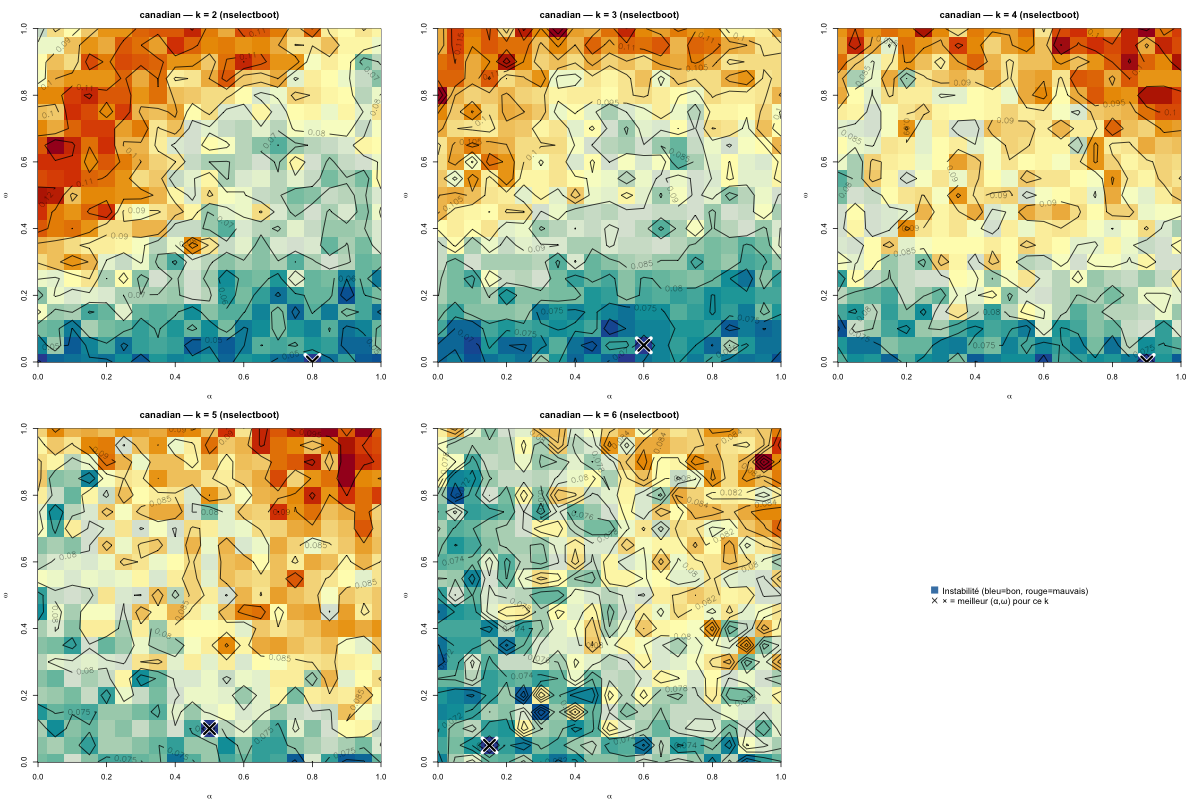
\includegraphics[width=0.85\textwidth]{figures/nselectboot_heatmap_canadian.png}
\end{center}

\subsection{AEMET}
\begin{center}
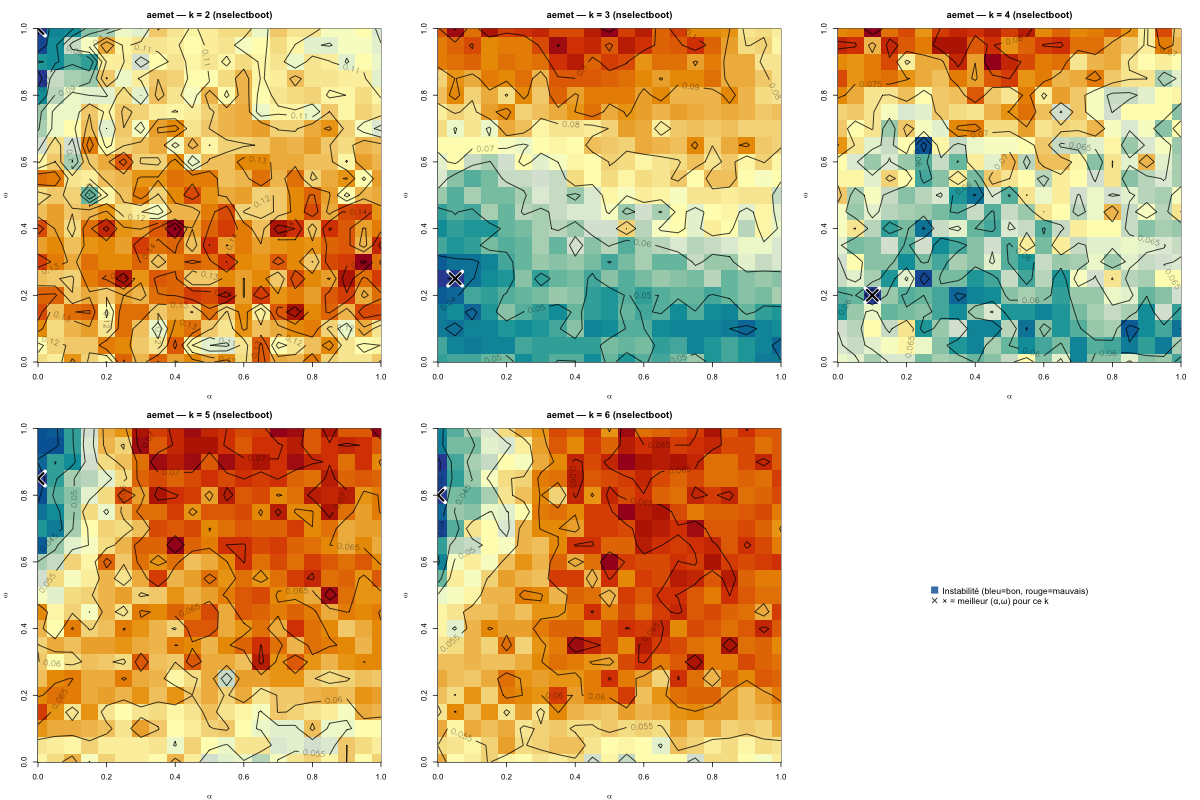
\includegraphics[width=0.85\textwidth]{figures/nselectboot_heatmap_aemet.png}
\end{center}

\subsection{Growth}
\begin{center}
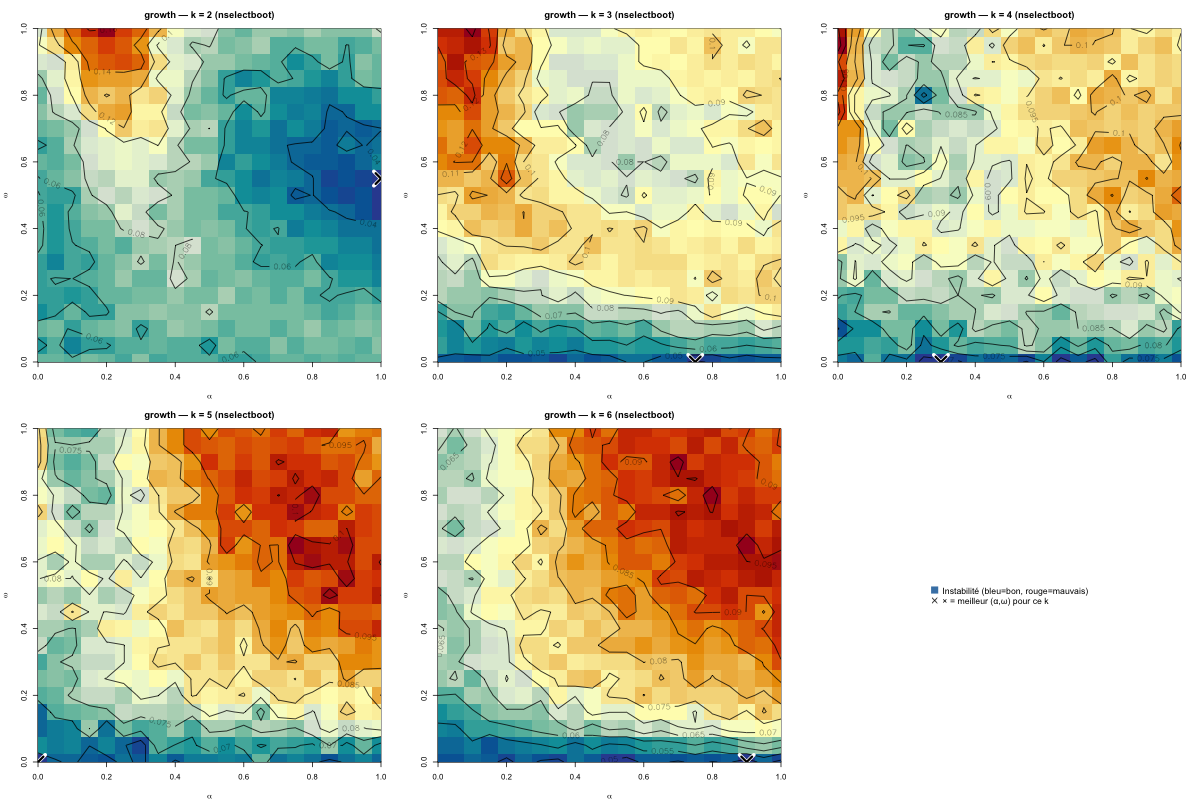
\includegraphics[width=0.85\textwidth]{figures/nselectboot_heatmap_growth.png}
\end{center}

\subsection{Tecator}
\begin{center}
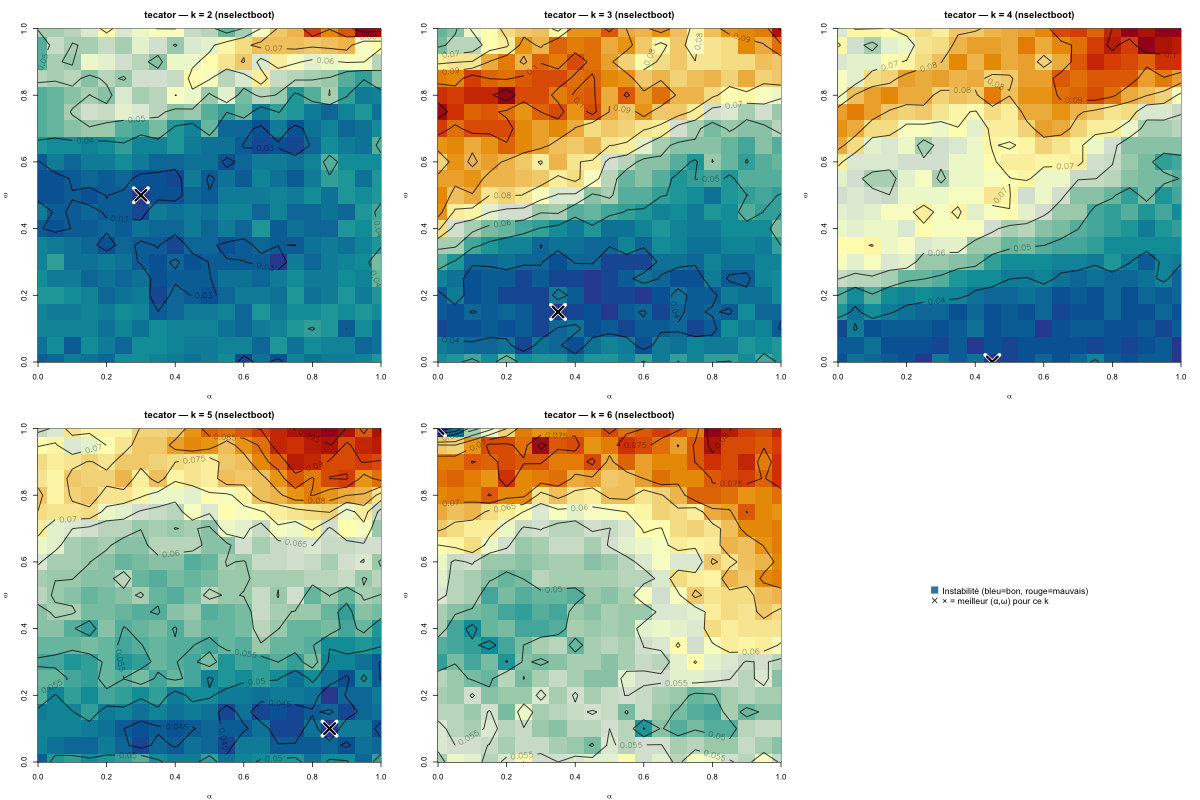
\includegraphics[width=0.85\textwidth]{figures/nselectboot_heatmap_tecator.png}
\end{center}

% ============================================================================
\section{Volet simulé (complément contrôlé)}
% ============================================================================

On enrichit l'expérience~1 avec le \textbf{même} type de procédure nselectboot
appliquée aux \textbf{données simulées} du projet (Cas2\_deriv, scénarios S1--S4
comme l'expérience~03). Ici $k_{\mathrm{vrai}}$ et les labels sont fournis par le
générateur : l'intérêt est de \textbf{valider le pipeline} sous hypothèses
contrôlées, pas de conclure sur le monde réel sans les quatre jeux ci-dessus.

\paragraph{Risques et limites.}
\begin{itemize}
  \item Le générateur impose une structure de covariance et un couplage
    fonctionnel / vectoriel qui ne coïncident pas nécessairement avec les
    données réelles.
  \item Un nombre de seeds et de scénarios suffisant doit être documenté pour
    éviter tout cherry-picking (voir \texttt{results\_simulated/README.md}).
  \item Ce volet est explicitement \textbf{complémentaire} : les tableaux et
    heatmaps sur Canadian, AEMET, Growth et Tecator restent la référence
    empirique principale.
\end{itemize}

\paragraph{Synthèse numérique (seed référence = premier de \texttt{SEEDS\_SIM}, ici 1).}
Le fichier \path{results_simulated/nselectboot_simulated_summary_by_run.csv}
agrège, pour chaque (scénario, seed), la proportion de couples $(\alpha,\omega)$
pour lesquels $k_{\mathrm{opt}} = k_{\mathrm{vrai}}$, la médiane et le mode de
$k_{\mathrm{opt}}$ sur la grille. Les valeurs ci-dessous correspondent au
\textbf{dernier run versionné} (mode rapide : pas $0{,}2$ en $\alpha$ et $\omega$,
grille $6\times6$, $B=60$ ; orchestrateur \path{run_simulated_instabilite_only.R}).

\begin{table}[H]
\centering
\small
\begin{tabular}{lrrrrr}
\toprule
\textbf{Scénario} & \textbf{Seed} & $k_{\mathrm{vrai}}$ &
\textbf{Prop.\ }$k_{\mathrm{opt}} = k_{\mathrm{vrai}}$ &
\textbf{Médiane} $k_{\mathrm{opt}}$ & \textbf{Mode} $k_{\mathrm{opt}}$ \\
\midrule
S1 & 1 & 3 & 0{,}917 & 3 & 3 \\
S2 & 1 & 3 & 0{,}722 & 3 & 3 \\
S3 & 1 & 3 & 0{,}083 & 5{,}5 & 6 \\
S4 & 1 & 3 & 0{,}000 & 6 & 6 \\
\bottomrule
\end{tabular}
\caption{Volet simulé (\texttt{nselectboot\_simulated\_summary\_by\_run.csv}). Grille $6\times6$, $B=60$ ; pour une grille $21\times21$ et $B=150$ alignés sur les jeux réels, lancer \texttt{run\_simulated\_instabilite\_only.R -{}-full}.}
\label{tab:sim-summary}
\end{table}

\paragraph{Heatmaps (instabilité par $(\alpha,\omega)$ et $k$).}
Pour chaque scénario, une figure est produite par
\texttt{analyse\_nselectboot\_simulated.R} à partir des CSV
\texttt{nselectboot\_simulated\_S*\_seed*.csv}. Ci-dessous : seed~1, même run que
le tableau~\ref{tab:sim-summary}.

\HeatmapSim{S1}{1}

\HeatmapSim{S2}{1}

\HeatmapSim{S3}{1}

\HeatmapSim{S4}{1}

% ============================================================================
\section{Paramètres des expériences}
% ============================================================================

\begin{itemize}
  \item Grille $\alpha,\omega \in \{0, 0.05, \ldots, 1\}$ (21×21).
  \item $k \in \{2,\ldots,6\}$, $B=150$ répétitions bootstrap pour nselectboot.
  \item Même prétraitement que le pipeline principal :\\
    \path{src/01_lissage.R}, \path{src/02_fpca.R}, \path{src/03_distances.R}.
  \item \textbf{Simulé (mode par défaut du script orchestrateur) :} grille
    $6\times6$ en $(\alpha,\omega)$, $B=60$, $k\in\{2,\ldots,6\}$ ; sorties
    \texttt{experiments/01\_instabilite/results\_simulated/} et heatmaps
    \texttt{figures/nselectboot\_heatmap\_sim\_*.png}. Mode \texttt{-{}-full} :
    $21\times21$, $B=150$, aligné sur les quatre jeux réels.
\end{itemize}

% ============================================================================
\section{Conclusion}
% ============================================================================

L'expérience 1 s'appuie sur une méthode publiée (instabilité bootstrap, Fang \&
Wang) pour choisir $k$ à $(\alpha,\omega)$ fixé, puis explore toute la grille.
Les labels servent uniquement à l'ARI et aux matrices de confusion, pas au choix
de $(k,\alpha,\omega)$. Le volet simulé ajoute une validation sous modèle sans
se substituer aux résultats sur les quatre jeux réels.

\vspace{1em}
\noindent\textbf{Références :}
\begin{itemize}
  \item Fang, Y., Wang, J. (2012). Selection of the number of clusters via the
    bootstrap method. \textit{Computational Statistics and Data Analysis}, 56(3),
    468--477.
\end{itemize}

\end{document}
